\problemname{Drebėjimas kasyklose}
\illustration{.4}{img/Goodluck_Mine.jpg}{%
  \emph{Goodluck Mine, Passage} by Ashley Dace. 
  License CC BY-SA 2.0.}

\noindent
Apleistose Moravijos Nykštukų kasyklose įrengtos visiškai autonominės nedidukės alaus daryklos
išties yra Nykštukų inžinerijos išradingumo ir meistriškumo įrodymas!
Deja, kartais žemės drebėjimai niokoja kasyklas, dėl ko vamzdžiai išsiklibina ir iš piltuvų vertingasis skystis pilamas ant grindų.
Jūsų, kaip aukščiausiojo alaus daryklų saugumo prižiūrėtojo, pareiga yra išjungti mašinas visose kasyklų salėse, 
jeigu įvyktų žemės drebėjimas.

Keliauti tuneliais užtrunka laiko, todėl jūs neišvengiamai užtruksite atvykti prie daugelio mašinų.
Tačiau jūs norite, kad visas išpilto skysčio kiekis būtų kuo mažesnis.

\medskip
Nykštukų kasyklos sudarytos iš $n$~salių, sujungtų $n-1$~tunelių.
Visa kasyklų sistema yra jungi, tad iš bet kurios salės įmanoma pasiekti bet kurią kitą.
Pereiti tunelį užtrunka $1$~laiko vienetą.
Išjungti mašiną ir pereiti salę neužtrunka nė kiek laiko.
Jei kurioje nors salėje mašina išjungiama praėjus laikui~$t$ po žemės drebėjimo, ši mašina iš viso išpila
$t$~litrų skysčio.
Įvyksta lygiai vienas žemės drebėjimas, kuris paveikia visas sales tuo pačiu metu. 
Be to, jokia mašina negali būti išjungta prieš drebėjimą. 
Pradėti galite bet kurioje iš salių.

\section*{Pavyzdys}

Pirmojoje pavyzdinėje įvestyje (\emph{Sample Input~$1$}) aprašytos kasyklos atrodo štai taip:

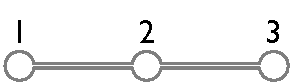
\includegraphics[width=.2\textwidth]{img/sample-1.pdf}

Jeigu pradėtumėte salėje~$2$ ir sales aplankytumėte tvarka $2$, $1$, $2$, $3$, 
tuomet mašinas išjungtumėte laiko momentu~$0$ (salėje $2$), laiko momentu~$1$ (salėje $1$) bei laiko momentu~$3$ (salėje $3$).
Iš viso būtų išpilstyta $0+1+3=4$~litrų skysčio.
Tačiau jeigu pradėtumėte salėje~$1$ ir sales aplankytumėte tvarka $1$, $2$, $3$, 
viso išpilsyto skysčio kiekis būtų $0+1+2=3$~litrų, kas yra geriau.

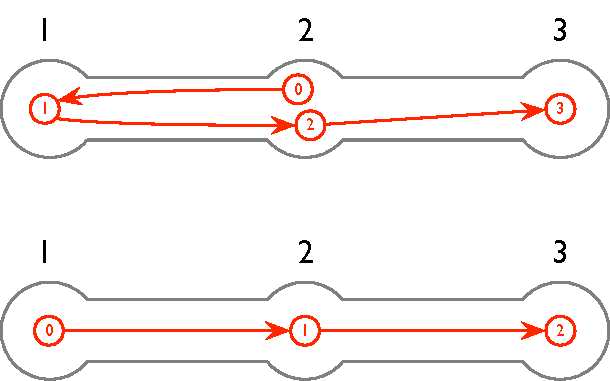
\includegraphics[width=.4\textwidth]{img/sample-1-ans.pdf}

\section*{Įvestis}

Pirmoje įvesties eilutėje pateiktas sveikasis skaičius $n$, žymintis salių skaičių.
Salės numeruojamos $1$, $\ldots$, $n$.
Kitose $n-1$ eilučių pateikiama po du sveikuosius skaičius $u$ ir $v$, kuriems galioja
$1\leq u < v \leq n$ % constraint:hallnames
ir kurie žymi, jog tarp salės~$u$ ir salės~$v$ yra tunelis.

\section*{Išvestis}

Išveskite vieną sveikąjį skaičių: kiek mažiausiai skysčio išsipils (litrais).

\section*{Ribojimai ir vertinimas}

Visada galios
$1\leq n\leq 10^5$. % constraint:n

Jūsų sprendimas bus testuojamas su keliomis testų grupėmis, kurių kiekviena verta tam tikro skaičiaus taškų.
Kiekviena testų grupė sudaryta iš įvairių testų.
Testų grupės taškai skiriami tik išsprendus visus testus, esančius toje grupėje.
Galutinis rezultatas lygus daugiausiai surinkusio sprendimo taškų skaičiui.

\medskip
\begin{tabular}{lll}
Grupė & Taškai & Papildomi ribojimai \\\hline
  $1$ & $18$ & jokia salė neturi daugiau nei dviejų tunelių\\
  $2$ & $19$ & daugiausiai viena salė turi daugiau nei du tunelius\\
  $3$ & $20$ & $n\leq 10$\\
  $4$ & $21$ & $n\leq 1000$\\
  $5$ & $22$ & \emph{Jokių papildomų ribojimų}
\end{tabular}
